\subsection{Ca sử dụng xem danh sách video recap}

\vspace{0.5cm}

\noindent 
\begin{tabularx}{\linewidth}{| l | X |} 
\hline 
\textbf{Mô tả} & Người dùng xem danh sách và trạng thái của các video đã tạo. \\
\hline 
\textbf{Luồng cơ bản} & 1. Người dùng bấm nút xem danh sách video ở thanh công cụ dưới màn hình. \newline
                       2. Hệ thống điều hướng đến trang danh sách video và hiển thị.\newline
                       3. Người dùng nhập tên album và bấm nút tạo album. \\
\hline 
\textbf{Hậu điều kiện} & - Người dùng có thể xem chi tiết trạng thái render của từng video. \newline
                        - Người dùng có thể xem những video đã render xong. \newline
                        - Hệ thống cập nhật trạng thái và tiến độ của các video trong thời gian thực. \\
\hline 
\textbf{Yêu cầu phi chức năng} & - Hệ thống lấy danh sách video không quá 2s. \newline
                        - Hệ thống cập nhật trạng thái video thời gian thực, không quá 0.5s. \\   
\hline 
\end{tabularx}

\vspace{0.8cm}

\noindent 
\begin{tabular}{| c | c |}
    \hline
    \textbf{Biểu đồ hoạt động} & \textbf{Quan hệ} \\ 
    \hline
    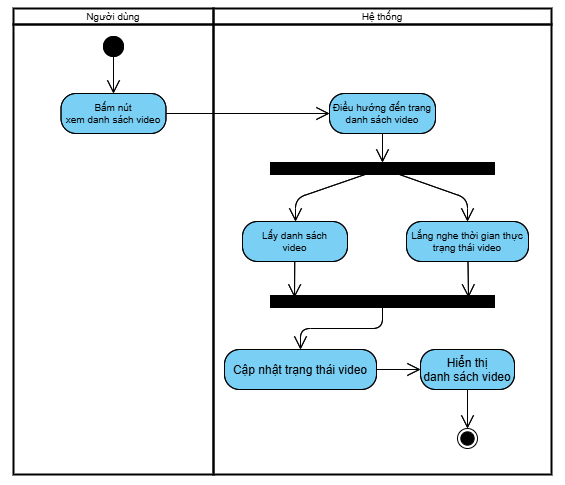
\includegraphics[width=0.6\linewidth]{figures/c3/3-3-8-activity-diagram.png} 
    &  
    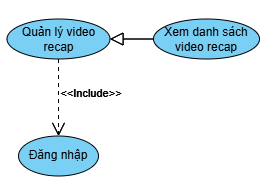
\includegraphics[width=0.35\linewidth]{figures/c3/3-3-8-relationship.png} \\ 
    \hline
\end{tabular}

\begin{figure}[H]
    \centering  
    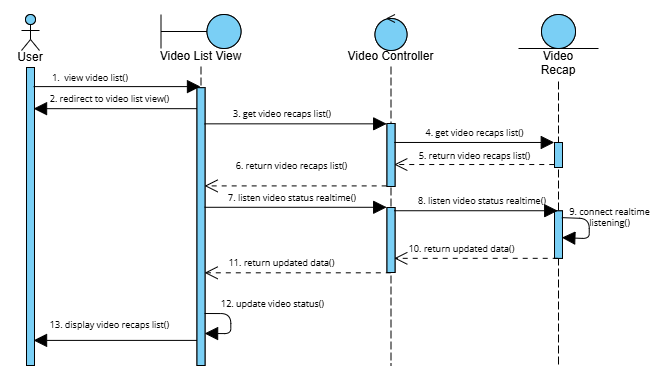
\includegraphics[width=1\textwidth]{figures/c3/3-3-8-sequence-diagram.png}
    \caption{Biểu đồ tuần tự ca sử xem danh sách video recap.}
    \label{fig:3-3-8-sequence-diagram}
\end{figure}